\chapter{关于本模板}

本模板以中国传媒大学研究生院《中国传媒大学研究生学位论文编写规则》为基础编写。

本模板为个人使用版本,并非官方认同的模板!切忌随意使用。

本人已使用该模板来编写毕业论文。

\section{二级标题示例}

\subsection{三级标题示例}

正文内容示例正文内容示例正文内容示例正文内容示例正文内容示例正文内容示例正文内容示例正文内容示例正文内容示例正文内容示例正文内容示例正文内容示例正文内容示例正文内容示例正文内容示例正文内容示例正文内容示例正文内容示例正文内容示例正文内容示例正文内容示例正文内容示例正文内容示例正文内容示例正文内容示例正文内容示例正文内容示例正文内容示例正文内容示例正文内容示例正文内容示例正文内容示例正文内容示例正文内容示例正文内容示例正文内容示例正文内容示例正文内容示例正文内容示例正文内容示例正文内容示例正文内容示例正文内容示例正文内容示例正文内容示例正文内容示例正文内容示例正文内容示例正文内容示例正文内容示例正文内容示例正文内容示例正文内容示例正文内容示例正文内容示例正文内容示例正文内容示例正文内容示例正文内容示例正文内容示例正文内容示例正文内容示例正文内容示例正文内容示例正文内容示例正文内容示例正文内容示例正文内容示例正文内容示例正文内容示例正文内容示例正文内容示例正文内容示例正文内容示例正文内容示例正文内容示例正文内容示例正文内容示例正文内容示例正文内容示例正文内容示例正文内容示例正文内容示例正文内容示例正文内容示例正文内容示例正文内容示例正文内容示例正文内容示例正文内容示例正文内容示例正文内容示例正文内容示例

正文内容示例正文内容示例正文内容示例正文内容示例正文内容示例正文内容示例正文内容示例正文内容示例正文内容示例正文内容示例正文内容示例正文内容示例正文内容示例正文内容示例正文内容示例正文内容示例正文内容示例正文内容示例正文内容示例正文内容示例正文内容示例正文内容示例正文内容示例正文内容示例正文内容示例正文内容示例正文内容示例正文内容示例正文内容示例正文内容示例正文内容示例正文内容示例正文内容示例正文内容示例正文内容示例正文内容示例正文内容示例正文内容示例正文内容示例正文内容示例正文内容示例正文内容示例正文内容示例正文内容示例正文内容示例正文内容示例正文内容示例正文内容示例正文内容示例正文内容示例正文内容示例正文内容示例正文内容示例正文内容示例正文内容示例正文内容示例正文内容示例正文内容示例正文内容示例正文内容示例正文内容示例正文内容示例正文内容示例正文内容示例正文内容示例正文内容示例正文内容示例正文内容示例正文内容示例正文内容示例正文内容示例正文内容示例正文内容示例正文内容示例正文内容示例正文内容示例正文内容示例正文内容示例正文内容示例正文内容示例正文内容示例正文内容示例正文内容示例正文内容示例正文内容示例正文内容示例正文内容示例正文内容示例正文内容示例正文内容示例正文内容示例正文内容示例正文内容示例

\section{示例}

\subsection{标题}

各级标题代码如 \ref{lst:各级标题示例代码} 所示。

\begin{lstlisting}[caption=各级标题示例 \LaTeX 代码,label=lst:各级标题示例代码]
    \chapter{一级标题}
    \section{二级标题}
    \subsection{三级标题}
    \subsubsection{四级标题}
    % 应该也用不着五级标题吧
\end{lstlisting}

\subsection{插图}

插图代码如代码 \ref{lst:插图示例代码} 所示。

\begin{lstlisting}[caption=插图示例 \LaTeX 代码,label=lst:插图示例代码]
\begin{figure}[!htb]    % 图片块
% !:允许排开文字, h:当前位置, t:页面顶部, b:页面底部, p:另开一页(不建议使用)
    \centering          % 居中
    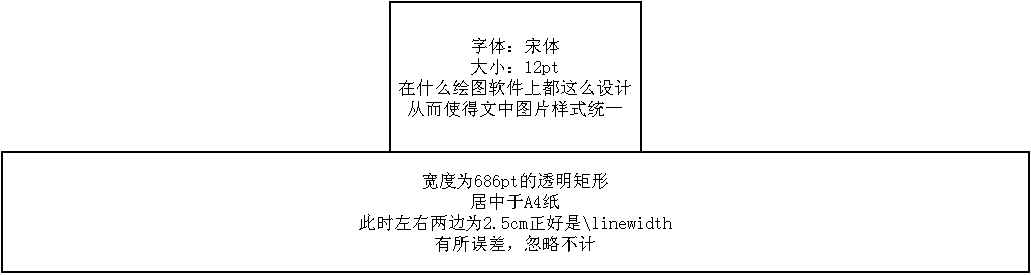
\includegraphics[width=\paperwidth]{示例图片.pdf} % 宽度、路径
    \caption{\label{fig:示例图片}示例图片} % 图片题注,引用
\end{figure}
% 引用:
\ref{lst:插图示例代码}
\end{lstlisting}

\begin{figure}[!htb]
    \centering
    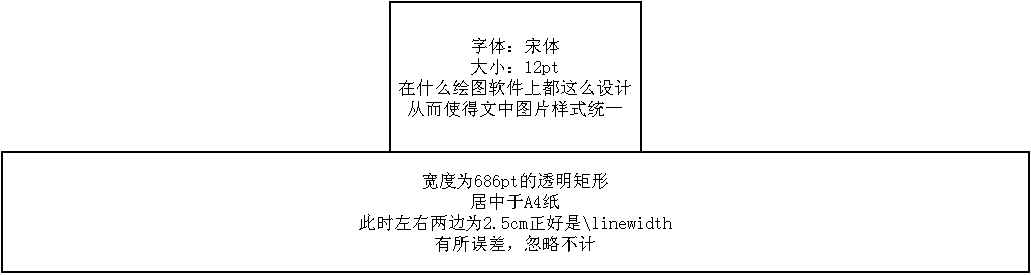
\includegraphics[width=\linewidth]{示例图片.pdf}
    \caption{\label{fig:示例图片}示例图片}
\end{figure}

\subsection{表格}

建议使用 \url{https://www.tablesgenerator.com/} 等在线制作表格的工具绘制表格,然后再对代码稍作修改。

普通的表格如表 \ref{tab:普通表格} 所示,代码如代码 \ref{lst:普通表格示例代码} 所示。

\begin{table}[htb] % 此处描述信息与图片块同
    \zihao{5} \songti % 表格样式 5号宋体
    \centering % 表格块居中
    \caption{普通表格} % 表头
    \label{tab:普通表格}
    \begin{tabular}{|l|l|l|}
        \hline
        \textbf{表头建议加粗} & \textbf{表头} & \textbf{表头} \\ \hline
        \textbf{左表头}       & 数据          & 数据          \\ \hline
        \textbf{左表头}       & 数据          & 数据          \\ \hline
    \end{tabular}
\end{table}

\begin{lstlisting}[caption=普通表格示例 \LaTeX 代码,label=lst:普通表格示例代码]
\begin{table}[htb] % 此处描述信息与图片块同
    \zihao{5} \songti % 表格样式 5号宋体 建议所有表格增加这句话
    \centering % 表格块居中
    \caption{普通表格} % 表头
    \label{tab:普通表格}
    \begin{tabular}{|l|l|l|}
        \hline
        \textbf{表头建议加粗} & \textbf{表头} & \textbf{表头} \\ \hline
        \textbf{左表头}       & 数据          & 数据          \\ \hline
        \textbf{左表头}       & 数据          & 数据          \\ \hline
    \end{tabular}
\end{table}
\end{lstlisting}

上述网站上一些拆分的功能都可以实现,表格拆分此处不给例子了。

若表头需要被斜线分割,则需使用diagbox宏包(已包含在packages.tex文件中),如表 \ref{tab:较为复杂的表格例子} 所示,是一个带有脚注和斜线分割表头的例子,代码如代码 \ref{lst:复杂表格示例代码} 所示。

\begin{table}[!htb]
    \zihao{-5} \songti \centering
    \caption{较为复杂的表格例子}
    \label{tab:较为复杂的表格例子}
    \begin{threeparttable}
        \begin{tabular}{|c|c|c|}
            \hline
            \diagbox{\textbf{分类1}}{\textbf{数据}}{\textbf{分类2}} & \textbf{表头1} & \textbf{表头2} \\ \hline
            \textbf{表头3}                                           & 数据1     & 数据2    \\ \hline
            \textbf{表头4}                                           & 数据3      & 数据4    \\ \hline
        \end{tabular}
        \begin{tablenotes}
            \footnotesize
            \item[*] 这里是脚注
        \end{tablenotes}
    \end{threeparttable}
\end{table}

\begin{lstlisting}[caption=复杂表格示例 \LaTeX 代码,label=lst:复杂表格示例代码]
\begin{table}[!htb]
    \zihao{-5} \songti \centering
    \caption{较为复杂的表格例子}
    \label{tab:较为复杂的表格例子}
    \begin{threeparttable}
        \begin{tabular}{|c|c|c|}
            \hline
            \diagbox{\textbf{分类1}}{\textbf{数据}}{\textbf{分类2}} & \textbf{表头1} & \textbf{表头2} \\ \hline
            \textbf{表头3}                                           & 数据1     & 数据2    \\ \hline
            \textbf{表头4}                                           & 数据3      & 数据4    \\ \hline
        \end{tabular}
        \begin{tablenotes}
            \footnotesize
            \item[*] 这里是脚注
        \end{tablenotes}
    \end{threeparttable}
\end{table}
\end{lstlisting}

如有其他形式的表格需要,请自行学习。

\subsection{代码}

行内代码 \verb|int main(){}|

\begin{lstlisting}[caption=代码示例,label=lst:代码示例]
行内代码 \verb|int main(){}|
\begin{lstlisting}[caption=代码示例,label=lst:代码示例]
end{lstlisting}
\end{lstlisting}

\subsection{引用}

参考文献引用:\cite{ref_example}

\begin{lstlisting}[caption=引用代码示例,label=lst:引用代码示例]
\ref{XXXX}
\cite{XXXX}
\end{lstlisting}

\verb|bib| 目录下有 \verb|reference.bib| 文件,内容形如:

\begin{lstlisting}[caption=引用代码示例,label=lst:引用代码示例]
    @misc{
        ref_example, # \cite命令后面跟着的名字
        title = {参考文献示例}, # 标题 
        authors = {AmnesiaBeing} # 作者
        XX = {YY} # 等等
    }
\end{lstlisting}

通常bib文件不要自行编写,最好使用文献管理工具生成,这样方便管理。

\subsection{公式}

LaTeX一大特色就是输入公式,不熟悉的情况下建议使用在线编辑器编辑然后复制回来,熟悉了就随意了。

\begin{equation}
    (I_{in}+jQ_{in})(I_{fir}+jQ_{fir})=(I_{in}I_{fir}-Q_{in}Q_{fir})+j(Q_{in}I_{fir}+I_{in}Q_{fir})
    \label{equ:complex_fir}
\end{equation}

\begin{lstlisting}[caption=引用代码示例,label=lst:引用代码示例]
\begin{equation}
    (I_{in}+jQ_{in})(I_{fir}+jQ_{fir})=(I_{in}I_{fir}-Q_{in}Q_{fir})+j(Q_{in}I_{fir}+I_{in}Q_{fir})
    \label{equ:complex_fir} % 公式也是可以有标签的
\end{equation}
\end{lstlisting}
